
\documentclass[a4paper,12pt]{report}

\usepackage[%
  russian,%
  an%
]{config}

\specialty{design_jocurilor}

\usepackage{longtable}
\usepackage{array}
\usepackage{ragged2e}
\usepackage{float}

\newcommand{\uniGroupName}{DJ2402}

\newcommand{\authorName}{MOSTAFA Mostafa}
\newcommand{\conducatorName}{Curmanschii Anton}
\newcommand{\conducatorTitleRo}{asistent universitar}

\newcommand{\authorNameRu}{MOSTAFA Mostafa}
\newcommand{\conducatorNameRu}{Curmanschii Anton}
\newcommand{\conducatorTitleRu}{ассистент университета}

\newcommand{\docTitleEng}{Designing a Multi-Agent AI Pipeline for Developing a Mobile Roguelite Game in Unity}
\newcommand{\docTitleRo}{Proiectarea unui pipeline multi-agent bazat pe inteligență artificială pentru dezvoltarea unui joc roguelite mobil în Unity}
\newcommand{\docTitleRu}{Проектирование мультиагентного AI-пайплайна для разработки мобильной roguelite-игры на Unity}

\newcommand{\yearOfWriting}{2026}
\newcommand{\conferencesList}{учебной защите курсовой работы, 2026~года}
\newcommand{\github}{\url{https://github.com/USER/REPO}}
\newcommand{\outputDate}{13.06.2026}

\newcommand{\aiUsage}{assisted}
\newcommand{\aiAssistanceExplanation}{Инструменты искусственного интеллекта использовались как объект исследования и как вспомогательное средство для проектирования, структурирования и проверки материалов. Итоговый текст и выводы проверены автором.}

\acro{AI}{Artificial Intelligence, искусственный интеллект}
\acro{API}{Application Programming Interface, программный интерфейс приложения}
\acro{BA}{Business Analyst, агент проверки требований и критериев приёмки}
\acro{GDD}{Game Design Document, документ игрового дизайна}
\acro{HUD}{Heads-Up Display, игровой экранный интерфейс}
\acro[ICT]{ICT/ИКТ}{Информационно-коммуникационные технологии}
\acro{LLM}{Large Language Model, большая языковая модель}
\acro{MCP}{Model Context Protocol, протокол подключения инструментов и внешних сред}
\acro{MVP}{Minimum Viable Product, минимально жизнеспособная версия продукта}
\acro{PM}{Project Manager, агент управления проектом и маршрутизацией}
\acro{PNG}{Portable Network Graphics, формат растровой графики}
\acro{QA}{Quality Assurance, агент проверки качества}
\acro{UI}{User Interface, пользовательский интерфейс}
\acro{UX}{User Experience, пользовательский опыт}

\setlength{\emergencystretch}{3em}
\sloppy
\graphicspath{{./images/}}

\hypersetup{hidelinks}
\newcommand{\file}[1]{\path{#1}}
\newcommand{\eng}[1]{\textit{#1}}
\newcolumntype{Y}{>{\RaggedRight\arraybackslash}X}

\begin{document}

\titlePage

\clearpage
\tableofcontents

\glsaddall
\acronymsChapter

\introChapter

Актуальность темы определяется быстрым развитием инструментов искусственного интеллекта, способных выполнять не только отдельные текстовые операции, но и комплексные проектные действия: анализировать требования, создавать документы, планировать архитектуру, генерировать ассеты, проверять ограничения и подготавливать задачи для реализации. В игровой индустрии такая возможность особенно важна, поскольку даже небольшой мобильный проект требует согласования игрового дизайна, интерфейсов, визуального стиля, технической архитектуры, тестирования и управления изменениями. При отсутствии формального процесса AI-инструменты могут создавать несвязанные результаты, противоречивые требования и трудно проверяемые артефакты. Поэтому практический интерес представляет не просто использование одной языковой модели, а построение контролируемого мультиагентного пайплайна, где каждый агент имеет роль, входные документы, ограничения и ожидаемый результат.

Объектом исследования является процесс разработки мобильной игры с применением AI-агентов. Предметом исследования является структура мультиагентного пайплайна, обеспечивающего разработку концепции, требований, UX/UI-спецификаций, ассетов и первичных Unity-артефактов для мобильной roguelite-игры.

Цель курсовой работы состоит в проектировании и анализе мультиагентного AI-пайплайна для разработки мобильной roguelite-игры на Unity на основе практического проекта «Евангелие Джекпота» / Gospel of the Jackpot.

Для достижения цели поставлены следующие задачи: исследовать теоретические основы AI-агентов и инструментального взаимодействия языковых моделей; определить роли агентов в игровом производственном процессе; описать архитектуру пайплайна, применённого в проекте; показать, какие игровые и технические артефакты были получены; оценить преимущества, ограничения и риски подхода; сформулировать рекомендации по дальнейшему развитию пайплайна.

Методологическую основу работы составляют анализ научных и технических источников по AI-агентам, инструментальным вызовам и мультиагентным системам, а также практическое моделирование процесса разработки игры через специализированные роли PM, GameDesigner, BA, UXDesigner, Architect, Coder, ArtDirector и QA. В качестве практической базы используется локальный проект с документами \file{AGENTS.md}, \file{STATUS.md}, \file{TASKS.md}, \file{GDD.md}, UX/UI-спецификациями, арт-манифестами, 78 сгенерированными PNG-ассетами и Unity UI prefab-файлами.

Теоретическое значение работы заключается в систематизации подхода, при котором AI-агент рассматривается не как универсальный чат-бот, а как специализированный участник производственного процесса с ограниченной ответственностью и проверяемыми результатами.

Прикладное значение состоит в том, что предложенная схема может быть использована для организации небольших игровых проектов, учебных прототипов и MVP-разработки на Unity.

Работа состоит из введения, трёх глав, заключительных выводов и рекомендаций, библиографии и приложений. Первая глава посвящена теоретическим основам AI-агентов и мультиагентных рабочих процессов. Во второй главе описывается проектирование игрового пайплайна и распределение ролей. В третьей главе анализируется практическая реализация пайплайна на материале проекта мобильной игры.

В рамках исследуемого проекта AI-инструменты рассматриваются как объект и средство проектирования игрового пайплайна: через них моделируются роли, передача задач, подготовка требований, UX/UI-спецификаций, арт-манифестов и Unity-артефактов. В курсовой работе анализируется именно эта проектная система и её результаты.

\chapter{Теоретические основы применения AI-агентов в разработке игр}

\section{Понятие AI-агента и отличие от обычного чат-бота}

В современных LLM-системах AI-агентом целесообразно считать приложение или программный процесс, который способен планировать действия, обращаться к инструментам, сохранять достаточный контекст и выполнять многошаговую задачу. В официальной документации OpenAI Agents SDK агенты определяются как приложения, которые планируют, вызывают инструменты, сотрудничают со специалистами и удерживают состояние, необходимое для завершения сложной работы \cite{openai-agents-sdk}. Такое определение важно для разработки игр, потому что игровой проект не сводится к генерации одного текста или одного фрагмента кода. Он состоит из последовательности решений, каждое из которых влияет на последующие этапы.

Обычный чат-бот отвечает на запрос пользователя преимущественно текстом. AI-агент, напротив, может быть включён в производственный контур: читать файлы проекта, применять правила репозитория, запускать команды, создавать документы, проверять результаты и передавать работу следующей роли. OpenAI описывает Codex как coding agent, который помогает писать код, понимать кодовые базы, проводить ревью, отлаживать проблемы и автоматизировать повторяющиеся задачи \cite{openai-codex}. Следовательно, в инженерном контексте агент ценен не только качеством текста, но и способностью действовать внутри существующей структуры проекта.

Для игровых проектов принципиально важно разделять генеративную способность модели и управляемость процесса. Языковая модель может предложить десятки игровых механик, но без роли аналитика, дизайнера, архитектора и тестировщика такие предложения останутся несогласованными. Мультиагентная схема решает эту проблему через распределение ответственности: один агент формирует дизайн, другой проверяет требования, третий переводит их в архитектурные задачи, четвёртый готовит ассеты, пятый контролирует качество.

\section{Инструментальные вызовы и структурированные результаты}

Ключевым техническим основанием агентного подхода является возможность связывать модель с внешними инструментами. В документации OpenAI function calling определяется как способ предоставить моделям доступ к новой функциональности и данным за пределами их обучающей выборки \cite{openai-function-calling}. Модель получает описание доступных инструментов, выбирает нужный инструмент, формирует аргументы вызова, а затем получает результат и продолжает работу. В разработке игр аналогом таких инструментов могут быть файловая система проекта, Unity MCP, генератор изображений, скрипты проверки, тестовые команды и системы задач.

Структурированные результаты также важны для надёжности. OpenAI указывает, что Structured Outputs позволяют получать ответы, соответствующие заданной схеме, и особенно полезны там, где результат должен быть обработан программно \cite{openai-structured-outputs}. В игровом пайплайне это проявляется в виде task card, manifest, acceptance criteria, asset\_id, target\_png\_path и других формальных полей. Если результат агента структурирован, его проще проверить, передать следующему агенту и использовать в Unity.

Научные исследования подтверждают значимость инструментального взаимодействия. Подход Toolformer показывает, что языковые модели могут обучаться выбирать внешние API и включать результаты вызовов в дальнейшее рассуждение \cite{toolformer}. Работа ReAct демонстрирует объединение рассуждения и действия: модель чередует reasoning traces и действия во внешней среде, что снижает ошибки и делает процесс более интерпретируемым \cite{react}. Эти идеи близки к практическому пайплайну разработки: агент не только пишет текст, но и действует в проектной среде, проверяет состояние и корректирует план.

\section{Мультиагентная координация}

Мультиагентная разработка предполагает, что одна сложная задача разделяется между специализированными агентами. В исследовании AutoGen мультиагентные приложения строятся через беседу нескольких настраиваемых агентов, которые могут сочетать LLM, инструменты и участие человека \cite{autogen}. Смежный пример агентного моделирования рассматривается в работе Generative Agents, где автономные агенты используются для имитации социального поведения \cite{generative-agents}. Это соответствует реальному производственному процессу, где результат одного специалиста становится входом для другого. Например, GameDesigner не должен сразу писать код, а Architect не должен создавать архитектуру без утверждённых требований.

В курсовом проекте мультиагентность была реализована не как свободная дискуссия агентов, а как жёсткий процесс с маршрутизацией. \file{AGENTS.md} задаёт правило: каждый агент перед началом читает свой манифест, статус проекта, очередь задач и входные файлы. Такой подход уменьшает вероятность случайных решений и делает процесс проверяемым. PM отвечает за маршрутизацию и состояние; GameDesigner формирует GDD; BA проверяет требования; UXDesigner создаёт UX/UI-спецификации; Architect переводит дизайн в технические задачи; Coder реализует Unity-артефакты; ArtDirector создаёт визуальные ассеты; QA проверяет соответствие.

Важным достоинством такой схемы является разделение полномочий. Если дизайн содержит неоднозначность, BA блокирует дальнейшую маршрутизацию. Если UX-спецификация не готова, Architect не начинает реализацию. Если ассеты не проверены, Coder не должен строить финальную интеграцию. Это напоминает классический производственный пайплайн, но ускоряется за счёт AI-агентов, которые способны быстро создавать черновики, находить противоречия и обновлять документацию.

\section{Специфика применения AI-агентов в game development}

Разработка игры отличается от разработки обычного информационного приложения тем, что здесь одновременно существуют механика, визуальный стиль, интерфейс, игровой ритм, техническая производительность и эмоциональный опыт игрока. В исследованиях по AI in games подчёркивается, что игровые AI-системы нужно оценивать не только технически, но и через взаимодействие с игроком и игровым опытом \cite{ai-and-games}. Даже MVP требует согласованности между GDD, UX, арт-пайплайном и кодом. Ошибка на раннем этапе может породить цепочку переделок: например, если дизайн допускает ручную кнопку possession, UX создаст кнопку, Coder реализует ввод, а QA позднее обнаружит конфликт с требованием movement-only.

AI-агенты полезны в game development именно там, где нужно быстро исследовать варианты и одновременно сохранять структуру. GameDesigner может предложить игровой цикл, BA может выявить недостающие acceptance criteria, ArtDirector может превратить стиль в стабильный prompt pack, а Architect может подготовить список prefab и систем. Но без ограничений AI-агенты склонны расширять scope, добавлять лишние функции, смешивать роли и генерировать непроверяемые решения. Поэтому в курсовом проекте использовались guardrails: MVP-состав, запрет на manual dash, запрет на manual possession button, запрет на manual slot spin, отсутствие IAP, ads и multiplayer в версии v1.

Таким образом, теоретический анализ показывает, что AI-агенты наиболее эффективны не как замена всей команды, а как ускорители отдельных производственных ролей. Их практическая ценность возникает при наличии контекста, инструментов, формальных входов и критериев приёмки.

\section{Выводы для главы 1}

AI-агент отличается от чат-бота способностью действовать в среде, использовать инструменты, удерживать состояние и выполнять многошаговые задачи. Для разработки игр наиболее рациональна мультиагентная схема, где роли разделены, результаты структурированы, а переходы между этапами контролируются правилами проекта.

\chapter{Проектирование мультиагентного пайплайна для мобильной roguelite-игры}

\section{Общая характеристика проекта}

Практической основой курсовой работы является проект мобильной roguelite-игры «Евангелие Джекпота» / Gospel of the Jackpot. Согласно GDD, игра проектируется как mobile-first roguelite в портретной ориентации для Android. Игрок управляет персонажем, который очищает заражённый культом мир, автоматически атакует ближайших врагов, временно вселяется в отмеченные сосуды и после каждой очищенной комнаты получает случайное благословение через автоматический сакральный слот-автомат.

Центральная дизайнерская ставка проекта строится на двух механиках: автоматический слот-автомат после комнат и временное автоматическое вселение во врагов. Эти механики создают сочетание риска, случайности и тактического движения. При этом управление намеренно упрощено под мобильный портретный формат: используется только floating joystick, атака выполняется автоматически, а possession запускается при полном заряде и приближении к отмеченному врагу.

Техническая цель MVP включает 5 боевых комнат и босса, целевую длительность забега 6-8 минут, reward pool из 12 стандартных карт и одного cursed deal, а также мета-разблокировку Broken Seal после первой победы. Проект ориентирован на Unity 2022 LTS, C\# и Android. Такой масштаб соответствует учебной курсовой работе: он достаточно мал для MVP, но содержит полный цикл проектирования от идеи до структурированных ассетов и UI-prefab файлов.

\section{Роли агентов и их ответственность}

В проекте была создана система AI-агентов, имитирующая небольшую игровую команду. В отличие от неформального использования чат-бота, каждый агент получил отдельную роль и набор входных документов. Это позволило организовать процесс как последовательность проверяемых handoff-файлов.

Распределение ролей агентов представлено в таблице 2.1.

\begin{table}[H]
\centering
\caption{Роли агентов и основные результаты их работы}
\small
\begin{tabularx}{\textwidth}{@{}p{0.19\textwidth}Y Y@{}}
\toprule
\textbf{Агент} & \textbf{Назначение} & \textbf{Основной результат} \\
\midrule
PM & Маршрутизация задач, контроль статусов, ведение TASKS и STATUS & Task cards, обновление статуса, handoff \\
GameDesigner & Проектирование игрового дизайна и MVP-механик & GDD, исправления требований \\
BA & Проверка требований, поиск неоднозначностей, acceptance criteria & Validation reports, blockers \\
UXDesigner & Проектирование мобильного UX/UI & UX/UI specs, wireframes, UI rules \\
Architect & Разделение дизайна на технические задачи & Implementation task cards, архитектурные решения \\
Coder & Создание Unity-артефактов и prefab & C\# / Unity prefabs \\
ArtDirector & Создание визуального стиля и prompt pack & Art bible, manifests, PNG assets \\
QA & Проверка соответствия acceptance criteria & QA reports, bug cards \\
\bottomrule
\end{tabularx}
\end{table}

Распределение ролей позволило применять правило dependency order: нельзя переходить к реализации без архитектурной задачи, нельзя создавать архитектурную задачу без UX-спецификации, нельзя формировать UX без валидированных требований. В \file{STATUS.md} видно, что проект несколько раз возвращался с этапа проверки требований к GameDesigner, когда BA находил неоднозначности. Такой возврат не является ошибкой процесса; напротив, он снижает стоимость будущих переделок.

\section{Документная архитектура пайплайна}

Пайплайн был организован вокруг файловой структуры. \file{AGENTS.md} задаёт общий протокол работы: определить роль, прочитать манифест, выполнить одну задачу, записать результат, при необходимости создать handoff и добавить запись в Sessions. \file{STATUS.md} фиксирует сделанное, активные задачи, следующие шаги и blockers. \file{TASKS.md} содержит таблицу задач от T00 до T21. \file{Tasks/Open} и \file{Tasks/Done} используются как очередь и архив выполненных handoff-карт.

Такой подход создаёт traceability: каждое решение можно связать с конкретной задачей, агентом и причиной. Например, BA заблокировал прямую архитектурную маршрутизацию из-за неоднозначности possession-explosion. GameDesigner уточнил поведение как buff-only explosion через P03 Last Breath. Затем BA повторно подтвердил, что default possession exit не создаёт explosion VFX, area damage, extra token или pickup, а P03 является единственным источником такого эффекта. Это решение затем перешло в UX-спецификации и арт-правила.

Основные файлы и папки пайплайна приведены в таблице 2.2.

\begin{table}[H]
\centering
\caption{Документная архитектура мультиагентного пайплайна}
\small
\begin{tabularx}{\textwidth}{@{}p{0.36\textwidth}Y@{}}
\toprule
\textbf{Файл/папка} & \textbf{Функция в пайплайне} \\
\midrule
\file{AGENTS.md} & Общий протокол агентов и порядок чтения контекста \\
\file{GDD.md} & Единый источник игрового дизайна и MVP-границ \\
\file{STATUS.md} & Текущее состояние проекта, Done/In Progress/Next/Blockers \\
\file{TASKS.md} & Полная очередь задач и зависимости \\
\file{Tasks/Open} & Активные handoff-карты для агентов \\
\file{Tasks/Done} & История завершённых задач и проверок \\
\file{Assets/Generated/_ART_BIBLE} & Правила визуального стиля и Unity usage notes \\
\file{Assets/Generated/_MANIFESTS} & Манифесты ассетов, prompt pack и target paths \\
\file{Assets/Prefabs/UI} & Первичные Unity UI prefab-артефакты \\
\bottomrule
\end{tabularx}
\end{table}

\section{Игровые требования и UX-ограничения}

Наиболее важное решение проекта связано с мобильным управлением. Для Android portrait была выбрана модель movement-only: игрок управляет только движением через floating joystick. Атака, possession и запуск слот-машины не имеют отдельных боевых кнопок. Это решение уменьшает перегрузку экрана, улучшает one-handed play и соответствует ограничениям мобильного интерфейса.

UX-спецификация закрепляет несколько guardrails: все HUD и popup UI должны оставаться внутри safe area; нижняя левая зона отдана под joystick; центральная арена не должна перекрываться панелями; минимальная touch target зона составляет 48 dp equivalent; читаемый текст должен быть Unity UI text, а не частью сгенерированных изображений. В более поздней locked UX specification эти правила были конкретизированы через reference resolution 1080x1920, CanvasScaler match height, safe-area hierarchy, minimum touch target 96 reference pixels и запрет на lower-right combat buttons.

Эти решения согласуются с документацией Unity. Canvas Scaler с режимом Scale With Screen Size позволяет проектировать UI в заданном reference resolution и масштабировать его под разные размеры экранов \cite[Canvas Scaler]{unity-docs}. \file{Screen.safeArea} возвращает безопасную область экрана в пикселях и используется для предотвращения размещения интерфейса в невидимых или перекрытых областях дисплея \cite[Screen.safeArea]{unity-docs}. Unity Button предназначен для действий, выполняемых при click/release, поэтому в проекте подчёркнуто, что боевые HUD-индикаторы не должны быть кнопками, а реальные действия вроде Accept/Decline в cursed deal должны иметь корректные button hit areas \cite[Button]{unity-docs}.

\section{Арт-пайплайн и стабильные asset\_id}

Визуальная часть проекта была оформлена через Art Bible и manifest-driven pipeline. Стиль определён как stylized dark cartoon with grotesque religious-casino motifs. Основная палитра включает charcoal \#17151A, old gold \#C89B3C, wax white \#E8DCC2, crimson \#9E2431 и void violet \#6D4BC3. На рисунке 2.1 показана эта палитра, чтобы цвета были понятны визуально. Технические ограничения требуют PNG, прозрачный фон, читаемость на 64x64, отсутствие текста, букв, цифр, watermark, photorealism и 3D render.

\begin{figure}[H]
\centering
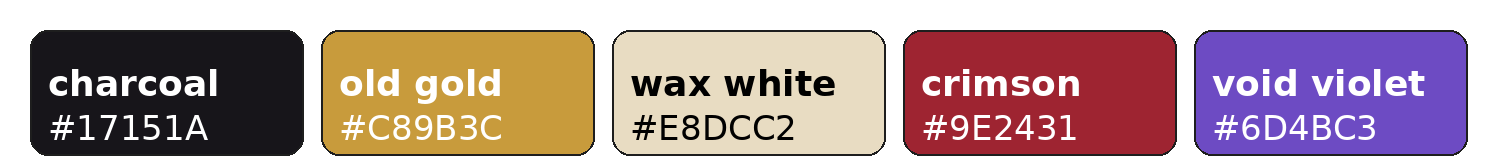
\includegraphics[width=0.84\textwidth]{palette.png}
\caption{Основная цветовая палитра визуального стиля проекта}
\end{figure}

Asset manifest содержит 78 строк, каждая из которых фиксирует asset\_id, target\_png\_path, prompt\_file\_path, folder, category, purpose, used\_by, required\_states, prompt, negative\_prompt, size, transparency и unity\_note. Такой формат делает генерацию ассетов воспроизводимой: ArtDirector не придумывает имена файлов, а сохраняет PNG строго в target path. Unity usage notes затем разделяют world SpriteRenderer assets, UI Image assets и overlay/VFX assets, указывая import settings, pivot и suggested prefab grouping.

Отдельно были введены hard visual restrictions. Slot machine body не должен содержать lever, handle, button или manual spin affordance, потому что игровой автомат является автоматической reward presentation, а не ручной casino-механикой. Это показывает, как дизайн-решение трансформируется в арт-ограничение и предотвращает неверную интерпретацию механики игроком.

\section{Критерии качества пайплайна}

Для оценки качества мультиагентного пайплайна недостаточно проверить только наличие файлов. Важно установить, насколько результаты связаны между собой и пригодны для дальнейшей реализации. В данном проекте можно выделить несколько критериев: трассируемость решений, отсутствие противоречий между документами, соблюдение MVP-границ, пригодность ассетов для Unity, мобильная читаемость интерфейса и наличие критериев приёмки для будущего QA.

Трассируемость означает, что каждое важное решение имеет источник. Например, запрет manual possession button появляется в GDD, затем повторяется в UX guardrails, затем закрепляется в ArtDirector restrictions и QA checklist. Такое повторение не является лишним: оно защищает проект от регрессии, когда на позднем этапе другой агент или разработчик случайно добавляет запрещённую кнопку.

Отсутствие противоречий проверяется через BA-итерации. Если GameDesigner формулирует механику неоднозначно, BA не должен пропускать документ дальше. В проекте это проявилось на примере possession-explosion: до уточнения нельзя было однозначно понять, является ли выход из possession атакой. После блокировки и доработки было зафиксировано, что default exit является non-damaging, а explosion относится только к reward P03.

Соблюдение MVP-границ проверяется через out-of-scope список. Для учебного проекта это особенно важно, потому что AI-агенты способны быстро расширить концепцию, но не всегда оценивают стоимость реализации. В проекте сознательно исключены несколько героев, procedural map, multiplayer, IAP, ads, branching routes и pet/helper system. Благодаря этому практическая часть остаётся достижимой для курсового масштаба.

Пригодность ассетов для Unity выражается в стабильных asset\_id, target\_png\_path, прозрачном фоне, запрете текста в PNG и указанных import settings. Если ассет содержит текст, его нельзя нормально локализовать; если путь нестабилен, Coder не сможет безопасно ссылаться на него; если silhouette нечитаема на 64x64, мобильный игрок не распознает объект. Поэтому Art Bible фактически выполняет роль технического договора между ArtDirector и Coder.

Мобильная читаемость интерфейса проверяется через locked UI rules. Reference resolution 1080x1920, safe-area hierarchy, minimum touch target, text hierarchy и запрет lower-right combat buttons образуют набор измеримых требований. Они позволяют оценивать UI не по вкусу, а по конкретным параметрам: размеру, положению, перекрытиям, читаемости и наличию ложных affordance.

\section{Выводы для главы 2}

Проектирование пайплайна показало, что AI-агенты должны работать не хаотично, а через формальные роли, документы, статусы, манифесты и критерии приёмки. Для мобильной игры особенно важны guardrails: ограниченный MVP, портретное управление, безопасная область UI, стабильные asset\_id и запрет на визуальные элементы, которые могут обещать несуществующие действия.

\chapter{Практическая реализация и анализ результатов}

\section{Последовательность работы пайплайна}

Практическая реализация началась с настройки проектного vault и первичной маршрутизации идеи к GameDesigner. Далее был создан initial GDD, после чего BA провёл проверку и выявил blocking design gaps. GameDesigner выполнил несколько итераций исправления, BA повторно проверял требования, а PM фиксировал изменения в \file{STATUS.md} и \file{TASKS.md}. Такая последовательность показывает, что AI-пайплайн не является одношаговой генерацией. Он работает итерационно: проектные гипотезы проходят проверку, возвращаются на доработку и только после утверждения переходят дальше.

Ключевые изменения требований касались control model, machine cadence, no-pet scope и possession-explosion ambiguity. Пользователь изменил модель управления, после чего BA открыл GDD заново. GameDesigner уточнил movement-only portrait controls, auto-attack и automatic marked-target possession. Позже BA заблокировал архитектурную маршрутизацию из-за machine cadence и possession explosion ambiguity. Только после уточнения, что default possession exit не является взрывом, а P03 Last Breath является единственным источником explosion feedback, GDD был утверждён для дальнейшей маршрутизации.

Ключевые итерации уточнения требований показаны в таблице 3.1.

\begin{table}[H]
\centering
\caption{Ключевые итерации практической работы пайплайна}
\small
\begin{tabularx}{\textwidth}{@{}p{0.25\textwidth}Y Y@{}}
\toprule
\textbf{Этап} & \textbf{Проблема} & \textbf{Решение} \\
\midrule
Initial GDD & Недостаточные требования и неоднозначности & BA validation и доработка GameDesigner \\
Control model & Риск перегрузки мобильного UI & Movement-only joystick, auto-attack, auto-possession \\
Machine cadence & Неясно, когда появляется reward machine & Автоматически после комнат 1-5 \\
Pet/helper scope & Расширение MVP & Полностью исключено из активного MVP \\
Possession explosion & Игрок мог ожидать взрыв по умолчанию & Default exit non-damaging; explosion только через P03 \\
UX routing & Architect не должен работать без UX & PM ввёл UXDesigner как обязательный этап \\
\bottomrule
\end{tabularx}
\end{table}

\section{Полученные проектные артефакты}

В результате работы пайплайна был получен набор артефактов, покрывающих основные стадии ранней разработки игры. GDD описывает игровой цикл, платформу, управление, системы MVP, bestiary, scenes, art style, acceptance criteria и out-of-scope features. UX/UI specification описывает combat HUD, possession marker, post-combat machine reward flow, cursed deal popup, victory/defeat results и first meta unlock presentation. Locked UX/UI specification фиксирует фактическое состояние Unity UI, safe-area правила, размер кнопок, текстовую иерархию и список required UI prefabs.

Арт-пайплайн произвёл 78 PNG-ассетов в \file{Assets/Generated}. Эти ассеты распределены по группам: characters, possession, slot\_machine, ui, environment и vfx. Для каждого ассета сохранены prompt file, negative prompt и Unity usage note. В \file{Assets/Prefabs/UI} присутствуют \file{GameOverRunSummaryScreen.prefab}, \file{GameplayHUD.prefab}, \file{MetaUnlockScreen.prefab}, \file{RewardScreen.prefab} и \file{SlotMachineResultScreen.prefab}. Это означает, что практическая часть не ограничилась концепцией: были сформированы реальные файлы, пригодные для Unity-интеграции.

Категории полученных артефактов приведены в таблице 3.2.

\begin{table}[H]
\centering
\caption{Категории полученных проектных артефактов}
\small
\begin{tabularx}{\textwidth}{@{}p{0.35\textwidth}Y@{}}
\toprule
\textbf{Категория результата} & \textbf{Примеры} \\
\midrule
Документы управления & \file{STATUS.md}, \file{TASKS.md}, Sessions \\
Игровой дизайн & \file{GDD.md}, revised control model, reward flow \\
Проверка требований & BA validation, blockers, acceptance criteria \\
UX/UI & Combat HUD, reward flow, cursed deal, results, meta unlock \\
Арт-документация & \file{style_rules.md}, \file{unity_usage_notes.md}, \file{asset_prompts.csv} \\
Ассеты & 78 PNG-файлов с прозрачным фоном \\
Unity UI prefab & GameplayHUD, RewardScreen, MetaUnlockScreen, SlotMachineResultScreen \\
\bottomrule
\end{tabularx}
\end{table}

\section{Анализ соответствия результата требованиям мобильной игры}

Для Android-проекта особенно важно, чтобы UI был читаемым, не перекрывал игровой центр и не создавал ложных affordance. В проекте это решено через портретную 9:16 структуру: верхняя safe-area band содержит HP, room progress и token count; possession charge размещён ниже; lower-left зона отдана floating joystick; lower-right зона намеренно пустая. Это соответствует UX-правилу, что player movement является единственным боевым input.

Наличие prefab-а GameplayHUD показывает, что HUD-подход уже материализован в Unity-файлах. RewardScreen и SlotMachineResultScreen отражают post-combat reward flow. MetaUnlockScreen связан с Broken Seal. Однако locked UX audit выявил и риски: button hit testing требовал проверки, RewardCard\_3 и RerollButton имели риск overlap, cursed deal modal нуждался в двух явных действиях Accept и Decline, а ResultsScreen должен получить один canonical implementation path. Эти замечания важны, потому что демонстрируют не только успех пайплайна, но и его способность находить недоработки до финального кодирования.

\section{Преимущества мультиагентного подхода}

Первое преимущество заключается в traceability. Каждое решение имеет источник: GDD, BA validation, UX spec, art rule или task card. Если в будущем возникнет вопрос, почему в игре нет manual possession button, ответ можно найти в GDD, UX guardrails и BA validation. Это снижает риск случайного возврата запрещённых механик.

Второе преимущество состоит в снижении scope creep. AI-модели часто предлагают дополнительные функции, потому что они стремятся сделать результат богаче. В игровом проекте это опасно: pet/helper system, multiplayer, IAP, ads, dash button или manual spin могли бы сильно увеличить объём работы. \file{AGENTS.md} и GDD явно фиксируют out-of-scope features, а BA следит, чтобы они не вернулись в MVP.

Третье преимущество - ускорение документационного цикла. В ручной разработке подготовка GDD, UX spec, art bible и task cards может занять значительное время. AI-агенты быстро создают черновики и варианты, а человек направляет процесс через правки и ограничения. При этом качество повышается не за счёт одной модели, а за счёт последовательной критики: BA проверяет GameDesigner, UXDesigner уточняет validated requirements, Architect строит задачи только после UX.

Четвёртое преимущество - формализация передачи между дисциплинами. ArtDirector получает не общее пожелание «сделать красиво», а manifest с asset\_id, prompt, negative prompt, size и target\_png\_path. Coder получает не свободное описание интерфейса, а список prefab, layout rules, touch target и запреты на hardcode. QA получает acceptance criteria, по которым можно проверять результат.

\section{Ограничения и риски}

Главный риск мультиагентного AI-пайплайна - ложная уверенность. Большой объём документов может создать впечатление завершённости, хотя игра ещё не полностью реализована и не протестирована на устройстве. В \file{STATUS.md} прямо указано, что Unity implementation остаётся gated by design/asset review, а пользователь должен вручную проверить сгенерированные sprites. Следовательно, документация не заменяет build, playtest и QA.

Второй риск - накопление ошибок в цепочке. Если ранний GDD содержит ошибочное требование, последующие агенты могут добросовестно развить эту ошибку в UX, art и code. Поэтому роль BA критична: она должна блокировать двусмысленность до того, как она станет дорогой. Пример possession explosion показывает, что один неясный эффект мог повлиять на VFX, damage logic, reward rules и player expectations.


\section{Рекомендации по дальнейшему развитию}

Для дальнейшей разработки рекомендуется перевести Architect handoff в конкретные Coder task cards: root Canvas ownership, button hit testing, reward overlap fix, cursed deal accept/decline, canonical ResultsScreen и MetaUnlockScreen. После этого Coder должен реализовать или исправить соответствующие Unity prefabs и связать их с gameplay state presenters. Затем QA должен выполнить portrait layout tests на 9:16, tall portrait, narrow portrait и safe-area/notch cases.

Также рекомендуется дополнить pipeline автоматическими проверками. Например, скрипт может проверять, что \file{asset_prompts.csv} содержит ровно 78 уникальных asset\_id, что все target\_png\_path существуют, что forbidden words вроде lever или manual spin не появляются в slot\_machine\_body prompt, что в UX-документах не появляются запрещённые combat buttons. Такой static validation усилит BA и QA и сделает процесс менее зависимым от ручного чтения.

Для масштабирования пайплайна можно добавить отдельного LocalizationAgent, который будет отвечать за Unity UI text и перевод терминов, а также BuildAgent, который будет запускать Unity build/test pipeline. Однако такие роли стоит добавлять только после стабилизации MVP, чтобы не нарушить принцип узкого scope.

\section{Матрица соответствия результатов цели работы}

Для проверки достижения цели полезно сопоставить поставленные задачи с фактическими результатами проекта. Такой способ оценки соответствует логике acceptance criteria, использованной в пайплайне. Если каждая задача имеет проверяемый результат, курсовая работа не превращается в описательный реферат, а демонстрирует практический вклад.

Сопоставление задач курсовой работы и полученных результатов приведено в таблице 3.3.

\begin{table}[H]
\centering
\caption{Матрица соответствия задач курсовой работы полученным результатам}
\small
\begin{tabularx}{\textwidth}{@{}p{0.34\textwidth}Y@{}}
\toprule
\textbf{Задача курсовой} & \textbf{Полученный результат} \\
\midrule
Исследовать AI-агентов & Описаны agents, tools, function calling, Structured Outputs, ReAct, Toolformer, AutoGen \\
Спроектировать роли & Определены PM, GameDesigner, BA, UXDesigner, Architect, Coder, ArtDirector, QA \\
Применить к игровому проекту & Пайплайн использован для Gospel of the Jackpot \\
Сформировать игровые требования & Создан и проверен GDD с MVP-границами \\
Сформировать UX/UI & Созданы mobile portrait specs и locked 9:16 rules \\
Подготовить ассеты & Создано 78 PNG-ассетов по manifest-driven pipeline \\
Оценить риски & Выявлены риски scope creep, ложной завершённости, ошибок цепочки и QA-зависимости \\
\bottomrule
\end{tabularx}
\end{table}

Матрица показывает, что результат работы имеет как теоретическую, так и практическую составляющую. Теоретическая часть объясняет, почему агентный подход применим к разработке. Практическая часть демонстрирует, что роли и документы были не только описаны, но и использованы для производства конкретных артефактов.

Отдельного внимания заслуживает критерий «готовность к реализации». Пайплайн не утверждает, что игра полностью готова. Он показывает переход от идеи к валидированным требованиям, UX/UI правилам, ассетам и первичным prefab. Следующий производственный этап должен быть посвящён Coder task cards, Unity-интеграции, сборке и QA. Такое разграничение важно для честной оценки результата.

\section{Предлагаемая методика QA для следующего этапа}

Следующий этап разработки должен включать систематическую проверку на уровне Unity. QA-агент должен проверить не только наличие экранов, но и соответствие поведения утверждённым правилам. Например, если combat HUD содержит joystick, QA должен убедиться, что он управляет только движением, не запускает атаку и не активирует possession. Если reward screen содержит reroll button, QA должен убедиться, что он доступен только в reward flow, а не в combat state.

Для проверки мобильного интерфейса рекомендуется использовать набор экранных конфигураций: базовый 9:16, высокий portrait screen, узкий portrait screen и устройство с safe-area/notch. В каждом случае проверяются верхний HUD, possession charge, joystick, reward cards, modal panels и result buttons. Любое перекрытие центральной арены, reward cards или bottom actions должно считаться bug candidate.

Для проверки игрового flow QA должен пройти несколько сценариев: обычная зачистка комнаты, появление reward machine после комнаты, использование reroll, stop-2 cursed deal accept, stop-2 cursed deal decline, possession default exit без explosion, possession exit с P03, defeat during possession и victory with first Broken Seal unlock. Такой набор сценариев покрывает наиболее рискованные места проекта.

Для проверки ассетов QA должен использовать не художественную оценку «нравится/не нравится», а технический checklist. PNG должен иметь прозрачный фон, не содержать букв и цифр, быть читаемым на 64x64, соответствовать asset\_id и target\_png\_path, не добавлять запрещённые механики. Например, если slot\_machine\_body\_idle визуально содержит lever, такой ассет должен быть отклонён даже при хорошем художественном качестве.

Автоматизация QA может быть добавлена постепенно. На первом уровне достаточно скрипта, который проверяет существование всех target\_png\_path из \file{asset_prompts.csv}. На втором уровне можно проверять уникальность asset\_id и соответствие папок. На третьем уровне возможно добавление визуальной проверки размеров PNG, альфа-канала и базовых импортных настроек. Такая автоматизация снижает ручную нагрузку и делает пайплайн воспроизводимым.

Дополнительно QA должен проверять не только конечные файлы, но и связь между решением и его источником. Для каждого спорного элемента полезно фиксировать цепочку: исходное требование, агент-исполнитель, артефакт, критерий приёмки и статус проверки. Например, отсутствие ручной кнопки possession должно быть подтверждено не одним документом, а сразу несколькими источниками: GDD, UX guardrails и BA validation. Такой подход упрощает защиту проектного решения и делает процесс менее зависимым от памяти разработчика.

Важной частью методики является разделение ошибок на design defect, implementation defect и asset defect. Design defect означает, что проблема находится в требовании или логике игры. Implementation defect относится к Unity-сценам, prefab, layout или обработчикам событий. Asset defect связан с PNG, prompt, размерами, прозрачностью или несоответствием стилю. Если все дефекты складываются в один общий список, команде сложнее понять, какой агент или человек должен исправлять проблему. Поэтому в следующей версии пайплайна целесообразно вести отдельные очереди задач для GameDesigner, UXDesigner, ArtDirector, Coder и QA.

Также следует использовать правило минимального изменения. Если QA обнаруживает проблему в RewardScreen, исправление не должно автоматически менять боевую механику, GDD или арт-стиль. Агент должен исправлять только тот участок, который связан с дефектом, и после правки показывать затронутые файлы. Это особенно важно в AI-пайплайнах, где одна генеративная правка может неожиданно изменить соседние решения. Ограничение diff scope повышает контролируемость и снижает риск регрессий.

Наконец, результаты QA должны возвращаться в проектную документацию. После проверки Unity-сборки статус каждого важного сценария можно перенести в \file{STATUS.md} или отдельный QA report. Тогда пайплайн будет не только создавать документы, но и поддерживать их актуальность после реализации. В долгосрочной перспективе это превращает репозиторий в единый источник истины для дизайна, интерфейса, ассетов, кода и проверки.

\section{Выводы для главы 3}

Практический проект подтвердил применимость мультиагентного AI-пайплайна для ранней разработки мобильной игры. Были получены GDD, UX/UI-спецификации, арт-манифесты, 78 PNG-ассетов и Unity UI prefab-артефакты. При этом подход требует обязательной проверки человеком, QA-тестирования и аккуратного контроля scope.

Материалы, вынесенные за пределы основного текста, приведены в приложениях: 1, 2, 3, 4 и 5.

\finalConclusionChapter

В результате выполнения курсовой работы была исследована и практически описана схема проектирования мультиагентного AI-пайплайна для разработки мобильной roguelite-игры на Unity. Цель работы достигнута: на основе проекта «Евангелие Джекпота» показано, как AI-агенты могут выполнять специализированные роли, создавать документы, проверять требования, формировать UX/UI-спецификации, готовить арт-манифесты и передавать результаты к Unity-реализации.

Теоретическая задача была решена через рассмотрение инструментальных вызовов, структурированных результатов и мультиагентной координации. Установлено, что AI-агент отличается от обычного чат-бота способностью использовать инструменты, удерживать состояние и выполнять многошаговые действия. Работы ReAct, Toolformer и AutoGen подтверждают актуальность подхода, в котором языковая модель не только генерирует текст, но и взаимодействует с внешними инструментами и другими агентами.

Проектная задача была решена через описание ролей PM, GameDesigner, BA, UXDesigner, Architect, Coder, ArtDirector и QA. Каждый агент получил ограниченную ответственность и входные документы, что позволило избежать смешения ролей и создать последовательность handoff-артефактов. Практическая задача была решена через анализ GDD, статусной таблицы задач, UX/UI-спецификаций, locked mobile 9:16 UI rules, art bible, asset manifest, 78 PNG-ассетов и UI prefab-файлов.

Практическая ценность полученного результата состоит в том, что предложенный пайплайн можно использовать как учебную и производственную модель для небольших игровых проектов. Он особенно полезен в MVP-разработке, где важно быстро пройти путь от идеи до проверяемых требований и первичных Unity-артефактов. Основная рекомендация заключается в сохранении жёсткого контроля над scope и требованиями: AI-агенты должны работать через документы, критерии приёмки и блокировки, а перед финальной реализацией необходимо провести ручной review ассетов, Unity integration review и QA-тестирование на реальных мобильных разрешениях.

Материалы курсового проекта доступны в GitHub-репозитории:
\url{https://github.com/1Mostafa23/ai-roguelite-pipeline-coursework}.

\bibliographyChapter

\appendixChapter

\section{Схема мультиагентного пайплайна}

\begin{center}
\textbf{Схема мультиагентного пайплайна}
\end{center}

\begin{tabularx}{\textwidth}{@{}p{0.13\textwidth}Y@{}}
\toprule
\textbf{Порядок} & \textbf{Передача} \\
\midrule
1 & Пользователь / PM $\rightarrow$ GameDesigner: идея игры и границы MVP \\
2 & GameDesigner $\rightarrow$ BA: GDD и игровые требования \\
3 & BA $\rightarrow$ GameDesigner: blockers или approval \\
4 & BA approval $\rightarrow$ UXDesigner: validated requirements \\
5 & UXDesigner $\rightarrow$ Architect: UX/UI specs and locked mobile rules \\
6 & Architect $\rightarrow$ ArtDirector: art generation task and manifest inputs \\
7 & ArtDirector $\rightarrow$ Coder: PNG assets and Unity usage notes \\
8 & Architect $\rightarrow$ Coder: implementation task cards \\
9 & Coder $\rightarrow$ QA: build/features ready for validation \\
10 & QA $\rightarrow$ PM: approval or bug cards \\
\bottomrule
\end{tabularx}

\section{Основные MVP-ограничения игры}

\begin{center}
\textbf{Основные MVP-ограничения игры}
\end{center}

\begin{tabularx}{\textwidth}{@{}p{0.28\textwidth}Y@{}}
\toprule
\textbf{Область} & \textbf{Зафиксированное решение} \\
\midrule
Платформа & Android, portrait orientation \\
Управление & Floating joystick only; no dash button \\
Атака & Automatic nearest enemy targeting \\
Possession & Auto-trigger only on marked vessel at full charge and range \\
Slot machine & Automatic post-combat reward presentation; no manual spin \\
Reward flow & Three reward cards, one choice, three rerolls per run \\
Cursed deal & Only on stop 2; +1 Attack, -1 Max HP \\
MVP run & 5 rooms plus boss, approximately 6-8 minutes \\
Out of scope & IAP, ads, multiplayer, multiple heroes, pet/helper system \\
\bottomrule
\end{tabularx}

\section{Полученные asset-группы и визуальный результат}

Проектный архив содержит 78 PNG-ассетов в \file{Assets/Generated}, manifest-driven таблицу \file{asset_prompts.csv} и 5 Unity UI prefab-файлов. Скриншоты ниже показывают, что визуальный стиль, HUD, reward screen и портретная 9:16 композиция уже проверялись на игровом макете.

\begin{center}
\small
\begin{tabularx}{\textwidth}{@{}p{0.32\textwidth}Y@{}}
\toprule
\textbf{Группа} & \textbf{Назначение} \\
\midrule
Characters - Player & Player body, hit, death, empty shell, possessed overlay \\
Characters - Enemies & Weak cultist, fast fanatic, preacher states \\
Boss & Mother Couponella idle, hit, death and warning marker \\
Possession & Marked vessel ring, ready marker, active overlay, exit marker \\
Slot machine & Automatic machine body, reel panel, symbols \\
UI & HP, possession charge, tokens, reward cards, reroll, result panels \\
Environment & Corrupted village floor and props \\
VFX & Hit impact, death puff, possession tether, reward sparkle, P03 explosion \\
\bottomrule
\end{tabularx}
\end{center}

\begin{figure}[H]
\centering
\begin{minipage}{0.44\textwidth}
\centering
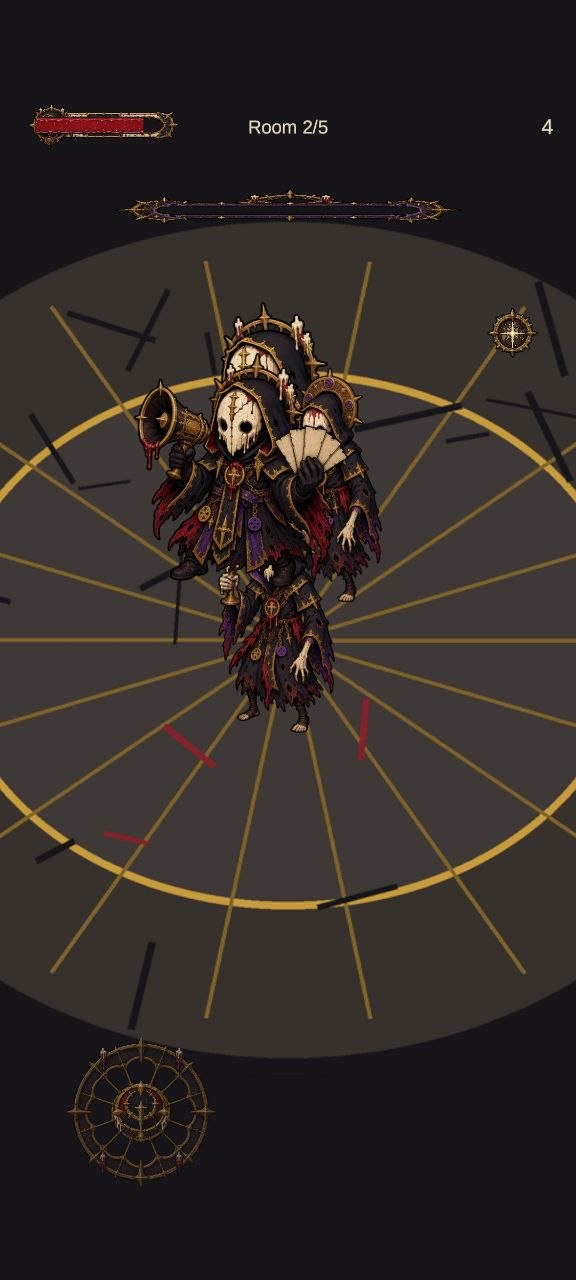
\includegraphics[height=0.43\textheight]{combat_hud.png}
\caption*{Combat HUD: room progress, HP, possession marker, joystick zone.}
\end{minipage}\hfill
\begin{minipage}{0.44\textwidth}
\centering
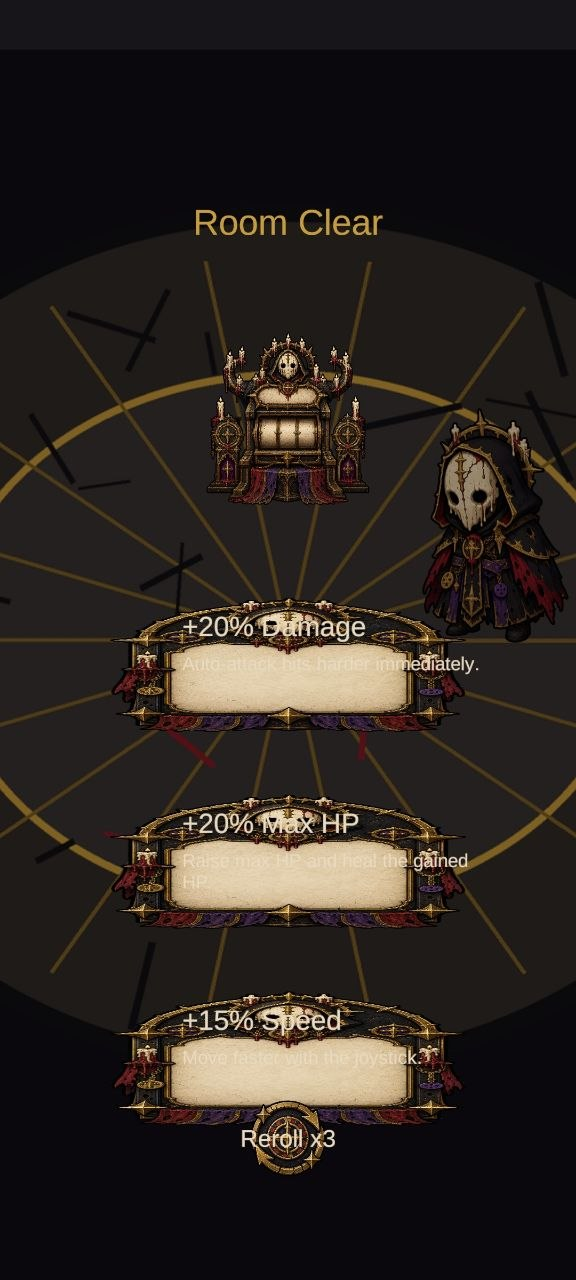
\includegraphics[height=0.43\textheight]{reward_screen.png}
\caption*{Room clear reward screen: 3 reward cards and reroll counter.}
\end{minipage}
\end{figure}

\section{Перечень manifest-listed asset\_id}

Ниже приведён исправленный перечень ассетов из \file{Assets/Generated/_MANIFESTS/asset_prompts.csv}. Колонка asset\_id заполнена реальными стабильными идентификаторами, по которым связываются prompt-файлы, PNG-выходы, Unity import settings и будущие prefab-ссылки. Проверка manifest показала: всего 78 строк, 78 уникальных asset\_id и 78 существующих target\_png\_path.

{\scriptsize
\setlength{\LTpre}{0pt}
\setlength{\LTpost}{0pt}
\renewcommand{\arraystretch}{1.0}
\begin{longtable}{@{}>{\RaggedRight\arraybackslash}p{0.38\textwidth}>{\RaggedRight\arraybackslash}p{0.23\textwidth}>{\RaggedRight\arraybackslash}p{0.35\textwidth}@{}}
\toprule
\textbf{asset\_id} & \textbf{Категория} & \textbf{Назначение} \\
\midrule
\endfirsthead
\toprule
\textbf{asset\_id} & \textbf{Категория} & \textbf{Назначение} \\
\midrule
\endhead
\path{player_body_idle} & Characters - Player & Default hero body, readable top-down/three-quarter silhouette. \\
\path{player_body_hit} & Characters - Player & Player hit feedback state. \\
\path{player_body_death} & Characters - Player & Player defeat/death visual. \\
\path{player_empty_shell_idle} & Characters - Player & Empty hero shell left in arena while possession is active. \\
\path{player_possessed_overlay_active} & Characters - Player & Overlay showing player is controlling a vessel. \\
\path{enemy_weak_cultist_idle} & Characters - Enemies & Weak cultist enemy base. \\
\path{enemy_weak_cultist_hit} & Characters - Enemies & Weak cultist hit state. \\
\path{enemy_weak_cultist_death} & Characters - Enemies & Weak cultist death state or last frame. \\
\path{enemy_fast_fanatic_idle} & Characters - Enemies & Fast fanatic enemy base. \\
\path{enemy_fast_fanatic_hit} & Characters - Enemies & Fast fanatic hit state. \\
\path{enemy_fast_fanatic_death} & Characters - Enemies & Fast fanatic death state or last frame. \\
\path{enemy_preacher_idle} & Characters - Enemies & Ranged preacher enemy base. \\
\path{enemy_preacher_hit} & Characters - Enemies & Preacher hit state. \\
\path{enemy_preacher_death} & Characters - Enemies & Preacher death state or last frame. \\
\path{boss_mother_couponella_idle} & Boss & Mother Couponella boss base sprite. \\
\path{boss_mother_couponella_hit} & Boss & Mother Couponella hit feedback. \\
\path{boss_mother_couponella_death} & Boss & Mother Couponella defeat sprite. \\
\path{boss_attack_warning_marker_ready} & Boss & Floor warning marker for boss AOE/tape attack. \\
\path{ui_hp_frame_idle} & Combat UI / HUD & HP bar frame. \\
\path{ui_hp_fill_active} & Combat UI / HUD & HP fill art. \\
\path{ui_possession_charge_frame_idle} & Combat UI / HUD & Possession charge bar frame. \\
\path{ui_possession_charge_fill_active} & Combat UI / HUD & Possession charge fill. \\
\path{ui_token_icon_idle} & Combat UI / HUD & Token currency icon. \\
\path{ui_room_progress_frame_idle} & Combat UI / HUD & Room progress frame. \\
\path{ui_room_progress_icon_active} & Combat UI / HUD & Active/cleared room progress token. \\
\path{ui_auto_attack_indicator_active} & Combat UI / HUD & Optional indicator that auto-attack is active. \\
\path{ui_auto_attack_indicator_disabled} & Combat UI / HUD & Optional inactive auto-attack indicator. \\
\path{ui_joystick_base_idle} & Touch Controls & Floating joystick base at rest. \\
\path{ui_joystick_base_active} & Touch Controls & Floating joystick base while touched. \\
\path{ui_joystick_knob_idle} & Touch Controls & Floating joystick knob at rest. \\
\path{ui_joystick_knob_active} & Touch Controls & Floating joystick knob while dragged. \\
\path{possession_marked_vessel_ring_ready} & Possession & Ring showing valid marked vessel. \\
\path{possession_ready_marker_ready} & Possession & Marker that possession charge/proximity is ready. \\
\path{possession_active_overlay_active} & Possession & Active possession aura over controlled vessel. \\
\path{possession_exit_marker_active} & Possession & Non-damaging default possession exit marker. \\
\path{slot_machine_body_idle} & Slot Machine / Rewards & Sacred demonic slot machine body at rest. \\
\path{slot_machine_body_active} & Slot Machine / Rewards & Slot machine during automatic post-combat roll. \\
\path{slot_reel_panel_idle} & Slot Machine / Rewards & Reusable reel panel frame. \\
\path{slot_symbol_token_idle} & Slot Machine / Rewards & Reel token symbol. \\
\path{slot_symbol_candle_idle} & Slot Machine / Rewards & Reel candle symbol. \\
\path{slot_symbol_seal_idle} & Slot Machine / Rewards & Reel seal symbol. \\
\path{slot_symbol_eye_idle} & Slot Machine / Rewards & Reel eye symbol. \\
\path{ui_reward_card_frame_idle} & Slot Machine / Rewards & Standard reward card frame. \\
\path{ui_reward_card_frame_selected} & Slot Machine / Rewards & Selected reward card frame. \\
\path{ui_reward_card_frame_disabled} & Slot Machine / Rewards & Disabled/unavailable reward card frame. \\
\path{ui_reroll_icon_ready} & Slot Machine / Rewards & Reroll visual icon/button art. \\
\path{ui_reroll_icon_disabled} & Slot Machine / Rewards & Disabled reroll visual. \\
\path{reward_icon_standard_01} & Slot Machine / Rewards & Standard reward icon placeholder 01. \\
\path{reward_icon_standard_02} & Slot Machine / Rewards & Standard reward icon placeholder 02. \\
\path{reward_icon_p03_last_breath} & Slot Machine / Rewards & Standard reward icon for P03 Last Breath, the only possession-exit explosion source. \\
\path{reward_icon_standard_04} & Slot Machine / Rewards & Standard reward icon placeholder 04. \\
\path{reward_icon_standard_05} & Slot Machine / Rewards & Standard reward icon placeholder 05. \\
\path{reward_icon_standard_06} & Slot Machine / Rewards & Standard reward icon placeholder 06. \\
\path{reward_icon_standard_07} & Slot Machine / Rewards & Standard reward icon placeholder 07. \\
\path{reward_icon_standard_08} & Slot Machine / Rewards & Standard reward icon placeholder 08. \\
\path{reward_icon_standard_09} & Slot Machine / Rewards & Standard reward icon placeholder 09. \\
\path{reward_icon_standard_10} & Slot Machine / Rewards & Standard reward icon placeholder 10. \\
\path{reward_icon_standard_11} & Slot Machine / Rewards & Standard reward icon placeholder 11. \\
\path{reward_icon_standard_12} & Slot Machine / Rewards & Standard reward icon placeholder 12. \\
\path{ui_cursed_deal_frame_active} & Slot Machine / Rewards & Cursed deal card/popup frame. \\
\path{ui_cursed_deal_icon_fanatical_credit} & Slot Machine / Rewards & Icon for Fanatical Credit cursed deal. \\
\path{ui_victory_emblem_active} & Result Screens & Victory emblem after boss defeat. \\
\path{ui_defeat_emblem_active} & Result Screens & Defeat emblem. \\
\path{ui_game_over_panel_bg_idle} & Result Screens & Game over panel background decoration. \\
\path{ui_run_summary_frame_idle} & Result Screens & Decorative frame for run summary stats. \\
\path{ui_broken_seal_icon_idle} & Meta Unlock & First meta unlock icon: Broken Seal. \\
\path{ui_meta_unlock_panel_decoration_idle} & Meta Unlock & Meta unlock panel decoration. \\
\path{arena_floor_corrupted_village_idle} & Environment / Props & Simple arena floor/background for five combat rooms. \\
\path{prop_corrupted_village_house_idle} & Environment / Props & Corrupted village background prop. \\
\path{prop_altar_slot_machine_idle} & Environment / Props & Non-interactive altar slot-machine prop for arena dressing if needed. \\
\path{prop_sacred_casino_candles_idle} & Environment / Props & Casino-religious decorative candles. \\
\path{prop_casino_religious_banner_idle} & Environment / Props & Decorative banner without readable symbols. \\
\path{vfx_hit_impact_active} & VFX & Generic hit impact sprite. \\
\path{vfx_enemy_death_puff_active} & VFX & Enemy death puff. \\
\path{vfx_possession_tether_flash_active} & VFX & Possession tether/flash between player and vessel. \\
\path{vfx_reward_reveal_sparkle_active} & VFX & Reward reveal sparkle. \\
\path{vfx_cursed_deal_smoke_active} & VFX & Cursed deal smoke. \\
\path{vfx_p03_explosion_active} & VFX & P03 Last Breath damaging possession-exit explosion. \\
\bottomrule
\end{longtable}
}

\section{Календарный план дальнейшей реализации}

\begin{center}
\textbf{Календарный план дальнейшей реализации}
\end{center}

\begin{tabularx}{\textwidth}{@{}p{0.08\textwidth}p{0.37\textwidth}Y@{}}
\toprule
\textbf{№} & \textbf{Мероприятие} & \textbf{Ожидаемый результат} \\
\midrule
1 & Проверка сгенерированных PNG-ассетов пользователем & Список approved/rejected ассетов \\
2 & Создание Architect task cards для Unity-реализации & Очередь задач для Coder и QA \\
3 & Исправление UI button hit testing & Рабочие кнопки с корректной touch area \\
4 & Исправление RewardScreen overlap & Три reward cards и отдельная reroll zone \\
5 & Реализация CursedDealModal Accept/Decline & Модальное решение с двумя действиями \\
6 & Интеграция MetaUnlockScreen & Broken Seal появляется один раз после первой победы \\
7 & Проверка safe-area на Android portrait & Отчёт QA по layout cases \\
8 & Сборка MVP и playtest & Список багов и решений для следующей итерации \\
\bottomrule
\end{tabularx}

Данный календарный план не заменяет производственный backlog, но показывает логическую последовательность дальнейших работ. Сначала необходимо проверить визуальные ресурсы, затем закрепить технические задачи, после чего переходить к реализации и QA. Нарушение этой последовательности увеличивает риск переделок.

\declarationPage{}

\end{document}
